\chapter{\label{ch:trigg}UPC Trigger development for CMS}
  Rare physics process at the LHC require dedicated triggers in order to sort
    these processes from the billions of ordinary nucleus-nucleus collisions. 
  Unlike most heavy-ion triggers, UPC triggers are optimized for low-\pt{} 
    and low multiplicity events. 
  For this reason trigger development specific to UPC events was required to
    carry out the analysis in this thesis.

  The increase in collision rate of the LHC PbPb beams from 2010 to 2011 was
    nearly a factor of 15. 
  To accommodate this increase in rate, the 2011 trigger scheme needed to be 
    more selective than in 2010 where CMS could take any event which 
    appeared to have a collision.
  The available bandwidth was allocated equally amongst the various heavy ion
    analysis groups to pursue as wide a physics program as possible.
  From this consideration, bandwidth limits were placed on the trigger rates
    for each analysis group's trigger package. 
  
  \section{\label{sec:l1Trigger}L1 trigger}
    The UPC L1 triggers were designed to study UPC \JPsi{} production via the 
      dimuon and dielectron channels (see Section~\ref{sec:detTrg}).
    To achieve this, the loosest muon and electron triggers where combined with
      a trigger on energy in the ZDCs and no activity in BSCs (BSC veto).
    Additional triggers were commissioned in case radiation damage during the 
      run reduced the sensitivity of the BSCs.
    This required no activity in HF (HF veto). 
    These triggers are summarized in Table~\ref{tab:l1Triggers2011}.
    The ECAL2 and ECAL5 triggers in Table~\ref{tab:l1Triggers2011}
      indicate a 5 and 2 GeV threshold on $E_{T}$ measured in the ECAL.
    The MuonOpen trigger indicates that the trigger only 
      requires a muon candidate in one of the three muon sub-systems and that
      there is no momentum threshold.
    ZDC in the trigger names indicate energy constant with at least one neutron.
    The sign on the ZDC label indicates which of the two ZDCs is required. 

    \begin{table}[h]
      \centering
      \begin{tabular}{|l|l|l|l|l|}
        \hline L1 trigger name & Rate (Hz) & Prescale & Id & Type \\ \hline \hline
        MuonOpen and (ZDC$^{+}$~or~ZDC$^{-}$) and BSC veto & 2.1 & 1 & 1 & \multirow{3}{*}{Physics} \\  \hhline{----~}
        ECAL2 and (ZDC$^{+}$~or~ZDC$^{-}$) and BSC veto & 1.8 & 2 & 2 & \\  \hhline{----~}
        ECAL5 and (ZDC$^{+}$~or~ZDC$^{-}$) and BSC veto & 0.3 & 1 & 3 & \\  \hline
        (ZDC$^{+}$~or~ZDC$^{-}$) & 35 & 1500 & 4 & Monitor \\  \hline
        MuonOpen and (ZDC$^{+}$~or~ZDC$^{-}$) and HF veto & 0 & off & 5 & \multirow{3}{*}{Backup} \\ \hhline{----~}
        ECAL2 and (ZDC$^{+}$~or~ZDC$^{-}$) and HF veto & 0 & off & 6 & \\  \hhline{----~}
        ECAL5 and (ZDC$^{+}$~or~ZDC$^{-}$) and HF veto & 0 & off & 7 & \\  \hline
      \end{tabular}
      \caption{List of 2011 L1 seeds.}
      \label{tab:l1Triggers2011}
    \end{table}
    The cumulative L1 trigger rate for all the UPC L1 trigger seeds was
      required to be no greater than 200 Hz.
    This requirement comes from the need to keep the tracker read-out rate
      low. 
    The trackers baseline voltage can fluctuate due to the high tracker hit 
      multiplicities in PbPb collisions.
    In order to monitor the zero suppression of the tracker, the zero 
      suppression algorithm was executed using the HLT computing farm 
	      rather than in the tracker firmware.

    In order to record the efficiency monitoring data, the ZDC triggers were
      reduce to a lower rate by only keeping a fraction of the total trigger 
      rate. 
    The factor that the trigger rate is reduced by is called the prescale.
    A prescale of 2 for example means that half the triggers that were 
      accepted.
    If the prescale is set to 1, then whole trigger rate is accepted. 
    The prescales for the triggers were set to balance the competing objectives 
      of rate reduction and increasing the overlap between the monitoring and
      signal triggers.

  \section{\label{sec:hltTrigger}HLT trigger}
    An event must pass the selection criteria of an HLT path in order to be
      recorded. 
    As opposed to the L1 trigger, which has access only to information from
      calorimeters and muon chambers, the HLT has access to all of the CMS 
      sub-detectors including the tracker. 
    Reconstruction of a track in the pixel detector is used by the UPC 
      trigger paths.
    The use of the pixel detector only, as opposed to using the whole tracker 
      including the silicon strip detector, allows for quick track 
      reconstruction saving computing cycles.
    The UPC triggers were required to have at lease one reconstructed pixel 
      track in order to reject backgrounds where no particles are 
      reconstructed by the tracker.
    For the muon trigger in Table~\ref{tab:hltTriggers2011} the rate was 
      reduced by nearly a factor or 4 compared to its L1 seed rate in 
      Table~\ref{tab:l1Triggers2011}.
    \begin{table}[h]
      \centering
      \begin{tabular}{|l|l|l|l|l|l|}
        \hline HLT trigger  & Rate (Hz) & L1 prescale & HLT prescale & L1 seed & Type \\ \hline \hline
        L1UPCMuon and Pixel Track & 0.52 & 1 & 1 & 1 & \multirow{3}{*}{Physics} \\ \hhline{-----~} 
        L1UPCECAL2 and Pixel Track & 1.65 & 2 & 1 & 2 & \\ \hhline{-----~}
        L1UPCECAL5 and Pixel Track & 0.26 & 1 & 1 & 3 & \\ \hline
        L1ZDCOr & 3.6 & 1500 & 11 & 4 & \multirow{2}{*}{Monitor}  \\ \hhline{-----~}
        L1ZDCOr and Pixel Track & 2.8 & 1500 & 1 & 4 & \\ \hline
        L1UPCMuonHFVeto and Pixel Track & 0 & off & off & 5 & \multirow{3}{*}{Backup}   \\ \hhline{-----~}
        L1UPCECAL2HFVeto and Pixel Track & 0 & off & off & 6 & \\ \hhline{-----~}
        L1UPCECAL5HFVeto and Pixel Track & 0 & off & off & 7 & \\ \hline 
      \end{tabular}
      \caption{List of 2011 HLT trigger.}
      \label{tab:hltTriggers2011}
    \end{table}

    The total HLT output for the UPC trigger package was limited to 20 Hz. 
    The limiting factor for the HLT rate was the amount of disk space given 
      to this analysis. 
    To meet the bandwidth requirements and collect a significant sample
      of data for estimating efficiencies, the prescales were balanced with 
      the goal of achieving at least 5\% statistical precision on the 
      efficiency measurements. 
    As an example of the balancing of the prescales, the HLT  ZDC trigger that 
      did not require a pixel track was given a additional prescale factor 
      of 11 on the HLT.
    The ZDC path that also required a pixel track on the HLT, which used 
      the same L1 seed, was only prescaled at the L1.
    The prescale of 11 was set to ensure that at least 1000 of the pixel track 
      ZDC triggers overlapped with the ZDC L1 only triggers so that efficiency
      of the pixel track requirement in the trigger could be estimated from 
      the tracks lost.

  \section{Studies of 2011 PbPb data}
    The UPC triggers for the 2011 PbPb run make several studies possible.
    Three such studies are discussed below: $\gamma\gamma \rightarrow e^{+} 
      e^{-}$, UPC interactions in peripheral nuclear collisions, and forward
      UPC \JPsi{} using HF. 

    \subsection{High mass $\gamma\gamma \rightarrow e^{+} e^{-}$  in PbPb 2011}
      This measurement would make use of the electron triggers and combine the 
        current di-muon data with di-electron data from the ECAL triggers.
      Because of the smaller mass of the electron,
        di-electron production is slightly favor compared to di-muon 
        production.
      STARlight predicts that di-electron cross section is a factor of 
        2.5 higher in Xn break-up mode than for the di-muons channel when looking 
        at masses above 4 GeV.
      The ECAL is position just beyond the tracker, whereas the muon system is 
        the outermost sub-detector. 
      This elevates the main reduction of muon acceptance, which is the material
        budget. 

      The contribution from higher order diagrams can be explored by studying 
        photoproduction of di-lepton pairs.
      Because the Pb nucleus has a charge 82 times higher than the proton,
        the electromagnetic coupling is stronger, and therefore, higher
        order terms is the perturbative expansion would potentially be more 
        important.
      By measuring the cross section for $\gamma\gamma \rightarrow e^{+} e^{-}$,
        the extent to which higher order terms are needed in coherent photon
        coupling can be constrained. 
      Recent results by ALICE favor very small contributions for higher order
        terms \cite{}.
      In addition, this analysis provides a useful cross check to the UPC 
        quarkonia analysis such as \JPsi{} by verifying the cross section 
        normalization.

    \subsection{UPC hadronic overlap}
      In the model calculations for UPC quarkonia 
        photoproduction all hadronic interactions are rejected.
      However, inclusive \pt{} spectra of \JPsi{} measured by ALICE in 
        peripheral PbPb collisions show a low momentum peak consistent with 
        coherent photoproduction ~\cite{aliceIclJpsi}.
      \begin{figure}[h]
        \centering
        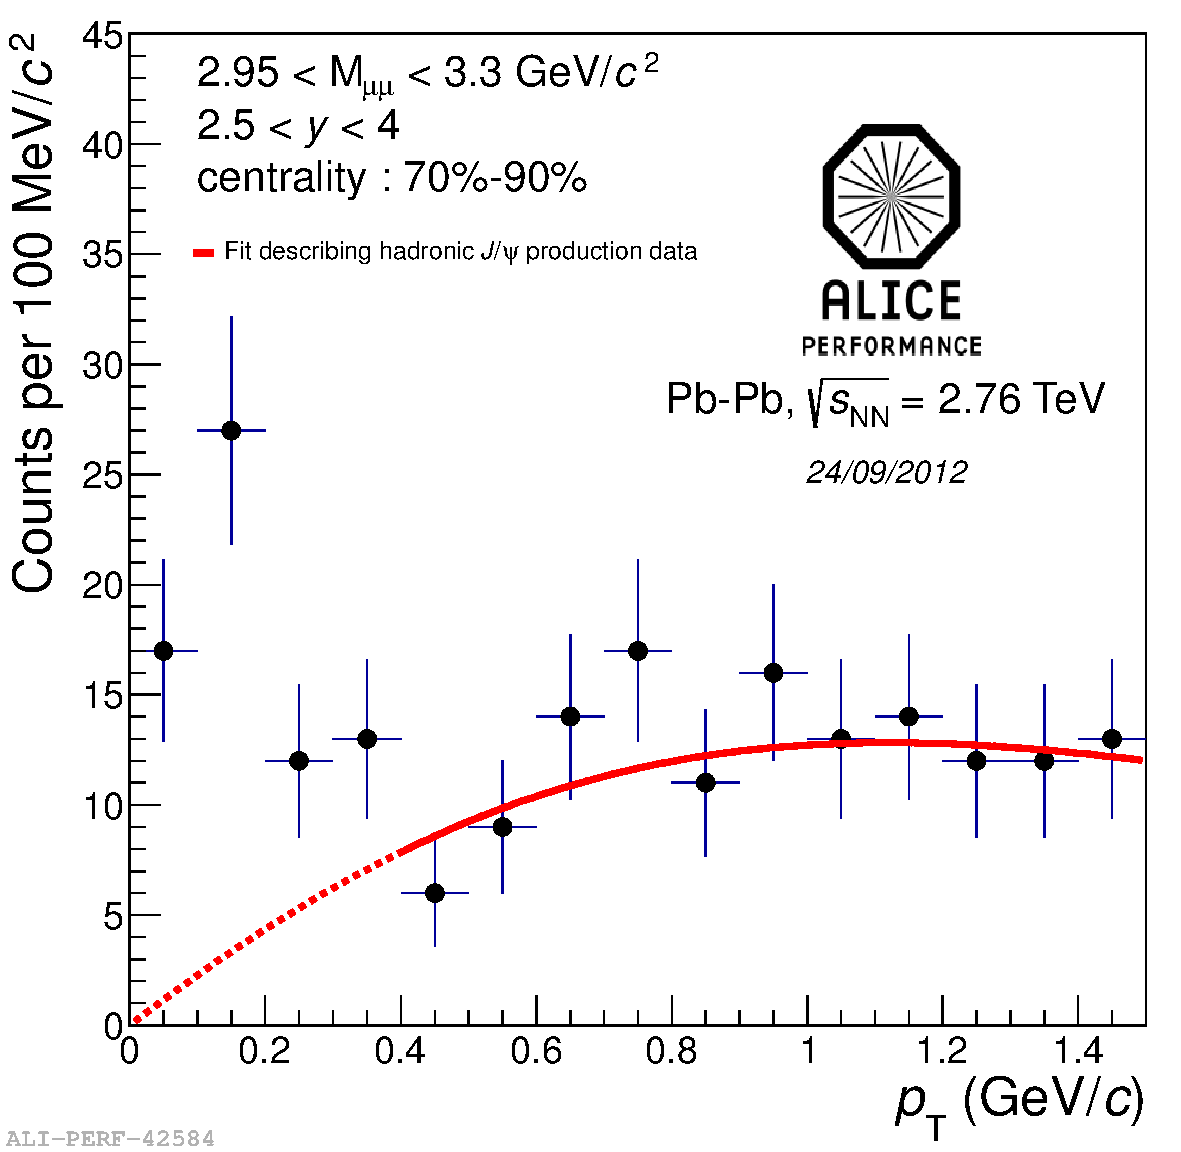
\includegraphics[width=0.5\textwidth]{2012-Sep-24-excess7090.pdf}
        \caption{Coherent excess in inclusive $J/\psi$ $p_{T}$ spectrum.}
        \label{fig:alicePtSpecLowPt}
      \end{figure}
      The ALICE spectra provide hints that UPC processes might also be present 
        in peripheral nucleus-nucleus collisions at the LHC.
      
      To study the overlap between photoproduction and hadronic production of 
        quarkonia eventi, the inelastic sample and the UPC sample could both be
        used. 
      The looseness of the rejection criteria to reject hadronic interactions,
        which uses the BSC detectors, leaves a significant overlap with 
        peripheral hadronic collisions. 
      The inclusive quarkonia sample from typical hadronic collisions can also 
        be utilized. 
      Coherent quarkonia photoproduction has a distinctive low $p_{T}$ structure
        that can be used to identify photoproduced candidates in a sample that 
        contains photoproduction combined with hadronic interactions.
      This measurement would open up the door to exploring the boundary between
        photoproduction and hadronic production.

    \subsection{UPC \JPsi{} with muons in HF}
      As higher rapidities are explored both lower and higher momentum partons
        of the nucleus are probed. 
      Because these two contributions to the UPC photoproduction cross section 
        can be separated using neutron tagging in incoherent events, exploring
        higher dimuon rapidities becomes attractive.
      HF extends to 5 in $\eta$, which is 2.6 units beyond the edge of the 
        tracker.
      By combining hits in HF with tracks in the tracker the higher dimuon 
        rapidities could be explored. 
      When combined with neutron tagging of incoherently produced quarkonia,
        the current study can be extended to probe lower-$x$ nuclear partons 
        by identifying muons in HF. 

 \section{\label{sec:pPbTrigDev}Trigger development for the LHC pPb Run}
   Specific UPC triggers were also developed for the pPb run in 2013. 
    For this period of running a much higher total trigger rate was read out 
      relative to 2011.
    The total rate allocated for UPC triggers at the L1 in 2013 was 5 kHz and 
      50 Hz at the HLT.
    This factor of 5 increase in HLT and factor of 25 in L1 bandwidth,
      allowed for a change in emphasis from the L1 to the HLT. 

    The basic strategy in 2013 was the same as in 2012, use the loosest 
      available ECAL and muon L1 triggers to push to capture the lowest \pt{}
      electrons and muons possible and reject hadronic interactions.
    Because of the L1 bandwidth restrictions in 2011, both the ZDCs and the 
      BCSs were used on the L1 to reduce rates.
    In 2013 only the muon and ECAL triggers were used on the L1 allowing for 
      rejection of hadronic interactions through cuts on track multiplicity. 
    In addition, a more sophisticated trigger using full dimuon reconstructed 
      was developed to increase purity.
    The main advantage in this shift in strategy was a higher purity due to 
      the increased sophistication of the reconstruction on the HLT.
    In addition, an increase in cross section of the underlying physics process
      was achieved by relaxing the neutron emission requirement.

    The HLT triggers in 2013 rejected hadronic interactions through counting
      tracks. 
    For the five UPC trigger paths included in the HLT menu, 
      three levels of reconstruction were done at the HLT.

    \begin{itemize}
      \item Pixel tracks were reconstructed from the inner pixel section of the 
        silicone tracker alone, tracks were reconstructed using the full
        tracker using the strips as well, and full dimuon reconstruction was 
        done using the tracker and muon detector. 
      \item The least restrictive pixel track paths required at least 
        one track reconstructed from the pixel detector and less than 10 pixel 
        tracks in the event.
      \item Full tracking paths were added on top of the pixel track paths and included
        an additional requirement of one full track and less than 7 reconstructed
        tracks.
      \item The most restrictive path added to the pixel and full tracking paths and 
        required reconstruction of dimuons with a mass between 2 and 12 GeV.
    \end{itemize}

    \subsection{pPb $J/\psi$}
      The CMS UPC triggers commissioned for the 2013 LHC pPb will allow for the
        study of \JPsi{} photoproduciton.
      This process is dominated $\gamma-p$ interactions \cite{}.
      The measurement would primarily probe the proton gluon densities.
      In Eq.~\ref{eq:photonFluxFinaltmp} the photon flux depends on the square
      of the number of protons in parent nucleus, $Z^{2}$. 
      However, the cross section of the target only increase as the total 
        number of nucleons to $A^{2/3}$.
      The much higher photon flux from the Pb-ion compensates for 
        the decreased size of the proton.

      A pPb UPC \JPsi{} measurement will complement the measurements done at 
        HERA \cite{}, and measurements done by ALICE \cite{}.
      CMS will contribute by adding additional kinematic coverage and cover a 
        unique range of $\gamma$p center of mass energies, $W_{\gamma p}$. 
      The difference in beam energies and species at LHC versus HERA result in
        access to different $W_{\gamma p}$. 
      ALICE and CMS have different acceptance in \JPsi{} rapidity, which also 
        translates to coverage of different $W_{\gamma p}$.
      In addition, an excess in the UPC cross section compared to HERA 
        measurements would indicate a non-exclusive contribution to the pPb UPC 
        \JPsi{} cross section. 
      This measurement will both help enhance the current understanding of 
        the $\gamma$p \JPsi{} photoproduction cross section as a function of 
        $W_{\gamma p}$.
